\startcontents[localtoc]
\printcontents[localtoc]{}{0}{\section*{Contents}\setcounter{tocdepth}{2}}



\phantomsection
\addcontentsline{toc}{section}{Overview}
\subsection*{Overview}



Sample data are simulated. QWTB is used to apply two different algorithms on the
same data. Uncertainty of the results is calculated by means of Monte Carlo
Method.



\phantomsection
\addcontentsline{toc}{section}{Generate sample data}
\subsection*{Generate sample data}



Two quantities are prepared: \texttt{t} and \texttt{y}, representing 0.5 second of sinus
waveform of nominal frequency 1 kHz, nominal amplitude 1 V and nominal phase
1 rad, sampled at sampling frequency \texttt{fsnom} 10 kHz.

\begin{lstlisting}
DI = [];
Anom = 1; fnom = 1e3; phnom = 1; fsnom = 1e4;
DI.t.v = [0:1/fsnom:0.5];
DI.y.v = Anom*sin(2*pi*fnom*DI.t.v + phnom);
\end{lstlisting}


Add noise of standard deviation 1 mV:

\begin{lstlisting}
DI.y.v = DI.y.v + 1e-3.*randn(size(DI.y.v));
\end{lstlisting}


\phantomsection
\addcontentsline{toc}{section}{Analyzing data}
\subsection*{Analyzing data}



To get a frequency spectrum, algorithm \texttt{SP-WFFT} can be used. This algorithm
requires sampling frequency, so third quantity \texttt{fs} is added.

\begin{lstlisting}
DI.fs.v = fsnom;
DO = qwtb('SP-WFFT', DI);
plot(DO.f.v, DO.A.v, '-xb'); xlim([980 1020])
\end{lstlisting}
\begin{lstlisting}[language={},xleftmargin=5pt,frame=none]
QWTB: no uncertainty calculation

\end{lstlisting}
\begin{center}
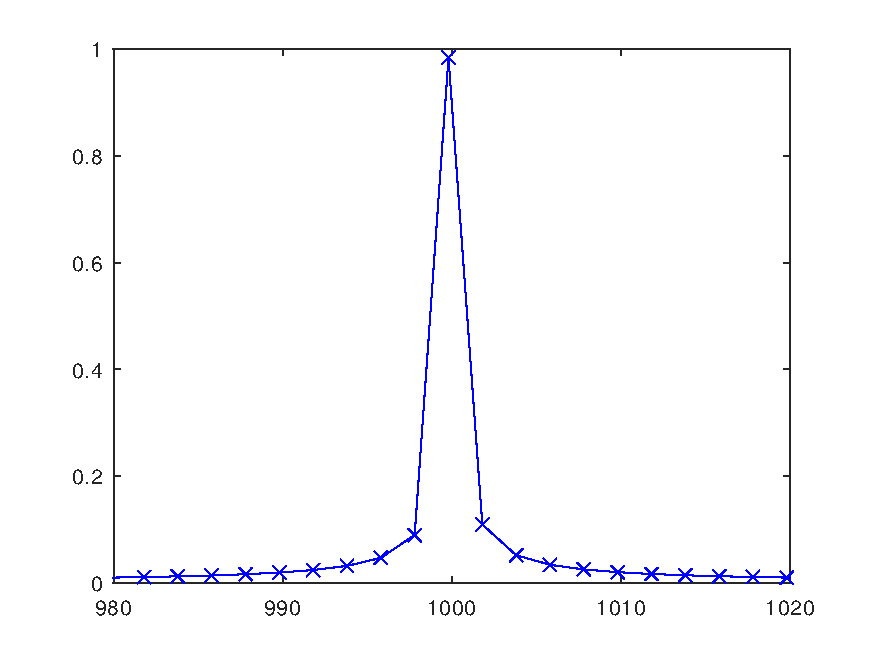
\includegraphics[width=0.7\textwidth]{qwtb_examples_published/qwtb_example_1-1.pdf}
\end{center}


One can see it is not a coherent measurement. Therefore to get 'unknown'
amplitude and frequency of the signal algorithm \texttt{PSFE} can be used:

\begin{lstlisting}
DO = qwtb('PSFE', DI);
f = DO.f.v
A = DO.A.v
\end{lstlisting}
\begin{lstlisting}[language={},xleftmargin=5pt,frame=none]
QWTB: no uncertainty calculation
QWTB: PSFE wrapper: sampling time was calculated from sampling frequency
f = 1000.0
A = 1.0000

\end{lstlisting}


\phantomsection
\addcontentsline{toc}{section}{Uncertainties}
\subsection*{Uncertainties}



Uncertainties are added to the \texttt{t} (time stamps) and \texttt{y} (sampled data) structures.

\begin{lstlisting}
DI.t.u = zeros(size(DI.t.v)) + 1e-5;
DI.y.u = zeros(size(DI.y.v)) + 1e-4;
\end{lstlisting}


Calculations settings is created with Monte Carlo uncertainty calculation
method, 1000 repeats and singlecore calculation. The output of messages is supressed to increase
calculation speed.

\begin{lstlisting}
CS.unc = 'mcm';
CS.mcm.repeats = 1000;
CS.mcm.method = 'singlecore';
CS.verbose = 0;
\end{lstlisting}


An uncertainty of sampling frequency has to be added. Let suppose the value:

\begin{lstlisting}
DI.fs.u = 1e-3;
\end{lstlisting}


Run PSFE algorithm on input data \texttt{DI} and with calculattion settings \texttt{CS}.

\begin{lstlisting}
DO = qwtb('PSFE',DI,CS);
\end{lstlisting}


Result is displayed as a histogram of calculated frequency (error from mean value multiplied by 1e6)

\begin{lstlisting}
figure; hist((DO.f.r - mean(DO.f.r)).*1e6, 50);
\end{lstlisting}
\begin{center}
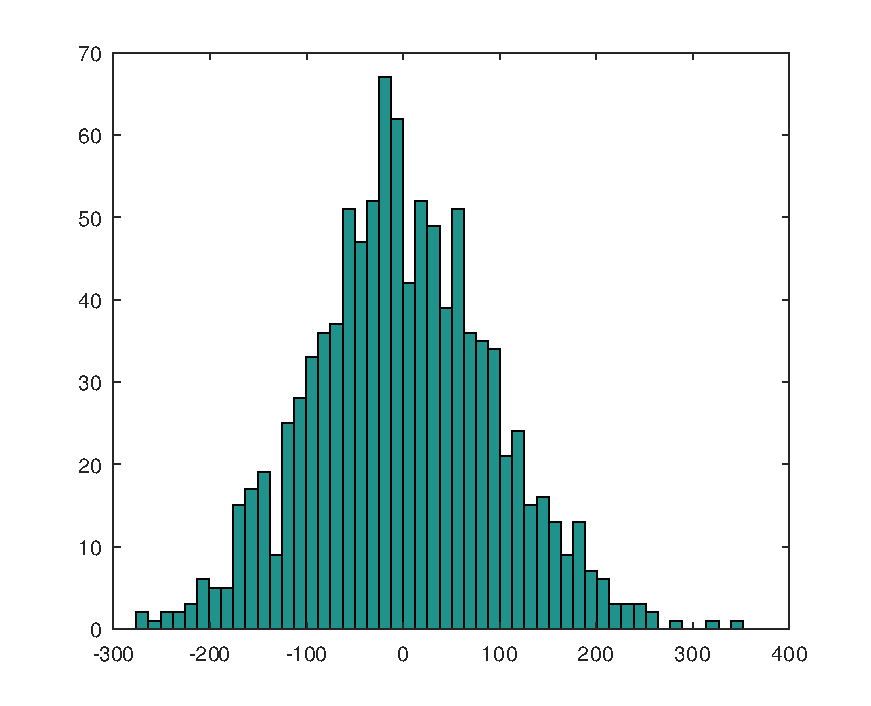
\includegraphics[width=0.7\textwidth]{qwtb_examples_published/qwtb_example_1-2.pdf}
\end{center}


One can see the histogram maybe is, maybe is not a Gaussian function. To get
correct uncertainties, a shortest coverage interval has to be calculated.



\stopcontents[localtoc]
